%\renewcommand{\thechapter}{5}
\chapter{Kinetic passive scalar advection by 2D velocity}
\label{chap:pp0}

\section{Introduction}
\label{pp0:sec:intro}

    Advection of a passive scalar by a turbulent velocity field is a fundamental and well
    studied problem in hydrodynamic turbulence \cite{obukhov49, corrsin51, batchelor59,
    kraichnan68, kraichnan74, kraichnan94, monin75, aref84, chaiken87, ottino89, zeldovich88, ott88, ott89, antonsen91, ramashankar91,
    solomon93, sreenivasan91,
    vanatta91, pierrehumbert94, antonsen95, frisch95, sreenivasan96, boratav97, lesieur97, shraiman00,
    warhaft00}. Investigations into passive scalar
    turbulence have helped develop the basic ideas underlying hydrodynamic turbulence
    theory (Refs.~\cite{sreenivasan91, shraiman00, warhaft00} give thorough reviews of this
    topic). 
    Recently, a few authors have carried out numerical investigations of passive scalar
    advection in magnetohydrodynamic turbulence \cite{maron01, busse08, mason14, sur14}. 
    However, to the best of our
    knowledge, kinetic passive scalar turbulence has not been studied before. 

    A kinetic passive scalar is 
    slaved to a turbulent cascade while simultaneously being phase mixed. Since the particle distribution functions for such
    systems may develop non-trivial velocity space structure, it is unclear if the results
    regarding passive scalar advection derived in the fluid limit will still be valid in the kinetic regime. 
    In the fluid limit, the passive scalar acquires the same
    energy spectrum as the advecting velocity field. However, in the kinetic limit, if
    phase mixing turns out to be the dominant process, the
    turbulent cascade of the scalar will terminate. This will result in an exponentially
    attenuated spectrum. The key question then is whether a kinetic passive scalar
    has a power law spectrum, or an exponentially decaying spectrum.
    
    The answer to this question has significant
    implications regarding how the system chooses to dissipate the energy contained in the
    scalar. There are two available dissipation mechanisms:
    phase mixing transfers energy to smaller
    velocity space scales, which eventually gets dissipated by collisions; on the other
    hand, the turbulent cascade transfers energy to small scales in real
    space, which is then dissipated by a diffusive term\footnote{Diffusion
    here is a stand-in for a more complicated cutoff like 
    finite Larmor radius effects. One may also consider it to be classical diffusion.}. In the context of KRMHD, all energy that is dissipated
    by collisions will end up heating ions, whereas the energy that survives in the low
    velocity moments until the cascade reaches the diffusive cutoff may end up heating
    either ions or electrons. Therefore, knowing how the injected energy gets
    partitioned between collisions and diffusion will shed some
    light on the differential heating of ions and electrons.

%    A
%    (simpler) system of particular interest is one where the velocity mixing the passive
%    scalar is fluid, while the
%    passive scalar itself is still kinetic---this is the case in the kinetic reduced MHD limit (the
%    $\EcrossB$ drift velocity is fluid-like, whereas the compressive fluctuations are
%    kinetic passive scalars). 
%
    In this chapter, we consider a simple model for a kinetic passive scalar $g$, which
    can be obtained from the KRMHD equation by making certain simplifying
    assumptions\footnote{This should be thought of as a first step towards solving the
    full KRMHD equations. Study of a simpler model such as this one helps develop understanding of
    how the full system behaves.} :
    \begin{enumerate}
        \item Electrostatic approximation: set $\delta \mb{B}_\perp = \hat{\mb{z}} \times
        \nabla \Apar = 0$.

        \item Assume the Kraichnan model~\cite{kraichnan94} for the velocity field, i.e.,
        let $\mb{u}_\perp$ be an Ornstein-Uhlenbeck process
        \cite{uhlenbeck30, chandrasekhar43, wang45, vankampen92,
        gardiner86, gillespie91, gillespie96, reif09} evaluated by solving the Langevin
        equation \cite{langevin1908}:
        \beq
            \pd{\Phi}{t} + \gamma \Phi = \kappa, \quad \mb{u}_\perp =
            \hat{\mb{z}}\times\nabla\Phi,
        \eeq
        where $\Phi$ is the stream function for the velocity field; $\kappa$
        is a white noise source, $\langle \kappa(t)\kappa(t')\rangle = \epsilon
        \delta(t-t')$. The amplitude of the advecting velocity (which can be thought of as
        the strength of the turbulence) is controlled by changing
        $\epsilon$. Depending on the value of $\epsilon$, $\gamma$ is chosen such that the
        Kubo number (a dimensionless parameter characterizing the correlation time of the
        velocity field) $\text{Ku}=p_\perp u_\perp/\gamma$, where $p_\perp$ is the
        perpendicular wavenumber of the velocity is held constant. We set $\text{Ku}=1$.
        
        \item Additionally, assume that the velocity field $\mb{u}_\perp$ is a 2D, single-scale velocity
        field, i.e., the energy containing wavenumbers $\mb{p}$ have $p_\perp\neq0,
        \ppar=0$.  Further assume that the scale given by $p_\perp$ corresponds to the
        largest scale (smallest magnitude wavenumber) in the system\footnote{In our
        numerical box, this corresponds to $p_\perp=1$.}---this is akin to the Batchelor limit
        \cite{batchelor59} in
        hydrodynamic turbulence. A cross section of the velocity field at constant $z$,
        along with the time evolution of the kinetic energy is plotted in
        \figref{pp0:fig:uperp}.
    \begin{figure}
    \begin{center}
        \includegraphics[width=7.4cm]{figs/phmixnlpp0/uperp.png}
        \includegraphics[width=7.4cm]{figs/phmixnlpp0/uperp_time.png}
        \caption{The velocity field $\mb{u}_\perp$ is independent of $z$. The structure 
        of the velocity field with respect to $x$ and $y$ is plotted on the left. The time
        evolution of the kinetic energy is plotted on the right.}
        \label{pp0:fig:uperp}
    \end{center}
    \end{figure}
    \end{enumerate}
    Under these assumptions the kinetic scalar \eqref{intro:krmhd:gpm} in KRMHD
    reduces to:
    \beq
     \partial_t g + \mathbf{u}_\perp \cdot \nabla_\perp g + \vpar \nabla_\parallel
     (g + \phi F_0) = C^h[g] + \eta \nabla_\perp^8 g + \chi, \label{pp0:eq:driftkin}
   \eeq
   \beq
     \phi  = \alpha \int_{-\infty}^\infty d \vpar g(\vpar),  \label{pp0:eq:boltz}
   \eeq
   where $\alpha$ is defined in the same way as \chapref{chap:phmixlin}, $\alpha = -1/\Lambda$ (see \eqref{intro:krmhd:Lambda}); 
   the electrostatic potential $\phi$ is same as the one used in \chapref{chap:phmixlin} (see
   \eqref{phmixlin:eq:phi}). $C^h[g]$ is the hyper-collision operator
   which in Hermite space looks like $-\nu m^8 g_m$ for the $m^{th}$ Hermite moment; $\eta
   k_\perp^8 g$ is a hyper-diffusion term that extracts energy from the system at small perpendicular scales
   in real space, and $\chi$ is a delta-correlated-in-time source term which drives $g$.
   Since \eqref{pp0:eq:driftkin} is homogeneous in $g$, the strength of $\chi$ can be set
   to one without any loss of generality.

\section{Nonlinear Cascade and timescales}
    \label{pp0:sec:timescales}
    
    Since the velocity $\mb{u}_\perp$ does not vary in the $z$, the passive scalar $g$ does not undergo a
    parallel cascade. This can be seen by considering a three mode interaction where modes with
    wavenumbers $\mb{p}$ and $\mb{q}$ couple to give a mode with the wavenumber $\mb{k} =
    \mb{q} + \mb{p}$. The parallel wavenumber remains unchanged, $\kpar = \qpar$. If the
    source $\chi$ injects energy into the system with a parallel wavenumber
    $k_{\parallel0}$ then the timescale
    associated with phase mixing is given by $(k_{\parallel0}\vth)^{-1}$.
    Since $p_\perp$ is non-zero, the passive scalar does get mixed in the
    perpendicular plane. The rate at which the scalar cascades to small perpendicular
    scales can be roughly estimated as $\sim |p_\perp u_\perp|$. 

    Since we have assumed that the scale of the velocity field is the largest scale in the
    system, we are in the so-called Batchelor limit \cite{batchelor59}; this implies that
    if $g$ were a fluid passive scalar
    instead of a kinetic one, it would have had a $1/k_\perp$ spectrum. On the other hand,
    if there were no velocity field, i.e., no turbulent cascade for the scalar, then the
    problem gets reduced to the one from
    \chapref{chap:phmixlin}, where the spectrum in velocity space is given by
    $1/\sqrt{m}$. In this sense, if the nonlinear cascade dominates over linear phase
    mixing, that corresponds to the ``fluid" limit, whereas in the ``kinetic" limit phase
    mixing is the dominant process.

\section{Numerical setup}
    We solved \eqsdash{pp0:eq:driftkin}{pp0:eq:boltz} using \Gand\,\footnote{\Gand\ has an
    option where instead of solving reduced MHD equations, it can be made to solve the Langevin
    equation to evaluate the velocity field $\mb{u}_\perp$. In this scenario $\epsilon$ and $\gamma$ are
    user-provided inputs which allow the user to control the strength of the velocity
    field.}. The velocity field was driven at wavenumbers $\mb{p}$ such that $p_\perp=1$,
    $\ppar=0$. The passive scalar $g$ was driven by injecting energy into the first Hermite
    moment at perpendicular wavenumbers between one
    and two, and parallel wavenumber $k_{\parallel0} = 1$. For these runs, we chose
    $\alpha=2$. As shown in \chapref{chap:phmixlin}, the particular value of $\alpha$ does
    not have any bearing on the Hermite space dynamics for $m\geq1$. It only determines the
    relationship between $g_0$ and $g_1$.
    The resolution
    was $64^2$ in the perpendicular plane, single wavenumber in the parallel direction and $100$ Hermite
    moments. We chose values for hyper-collision frequency $\nu$ and the hyper-difussion
    coefficient $\eta$, such that the collisional
    dissipation microscale was $m_c \sim 66$, and the
    diffusion microscale was $k_{\perp, \eta}\sim 21$\footnote{Due to the ``hyper" nature
    of the dissipation, the dissipation microscales give a better sense of the numerical
    setup, instead of the values of $\nu$ and $\eta$.}. 
    All the simulations in this chapter are in the ``strongly nonlinear" regime,
    \ie, in the limit where the nonlinear timescale is comparable to, or greater than the
    phase mixing timescale. In the opposite limit, phase mixing dominates and the problem
    reduces to the one discussed in \chapref{chap:phmixlin}.

   % The asymptotic Hermite spectra derived in \secref{phmixlin:sec:spectrum} assumed large
   % values of $\sqrt{m}$, suggesting that $\sqrt{m}\,$ is a more natural variable for our
   % model. 
    We change the Hermite space variable from $m$ to $s=\sqrt{m}$. 
    In terms of the new variables
    $(s, k_\perp, \kpar)$, the energy spectrum is given by $\Fsk = s |\gmk|^2$. The
    numerical results presented in this chapter use this definition for the energy
    spectrum.
    
    %The reasons for these choices become clearer later in
    %\chapref{chap:phmixnl}, for now it would suffice that $\Fsk$ is the energy spectrum of
    %the scalar,
    %i.e., the total free energy can be obtained by integrating $\Fsk$ over $s$, 
    %$k_\perp$ and $\kpar$.

\section{Results}
    
    \begin{figure}
    \begin{center}
        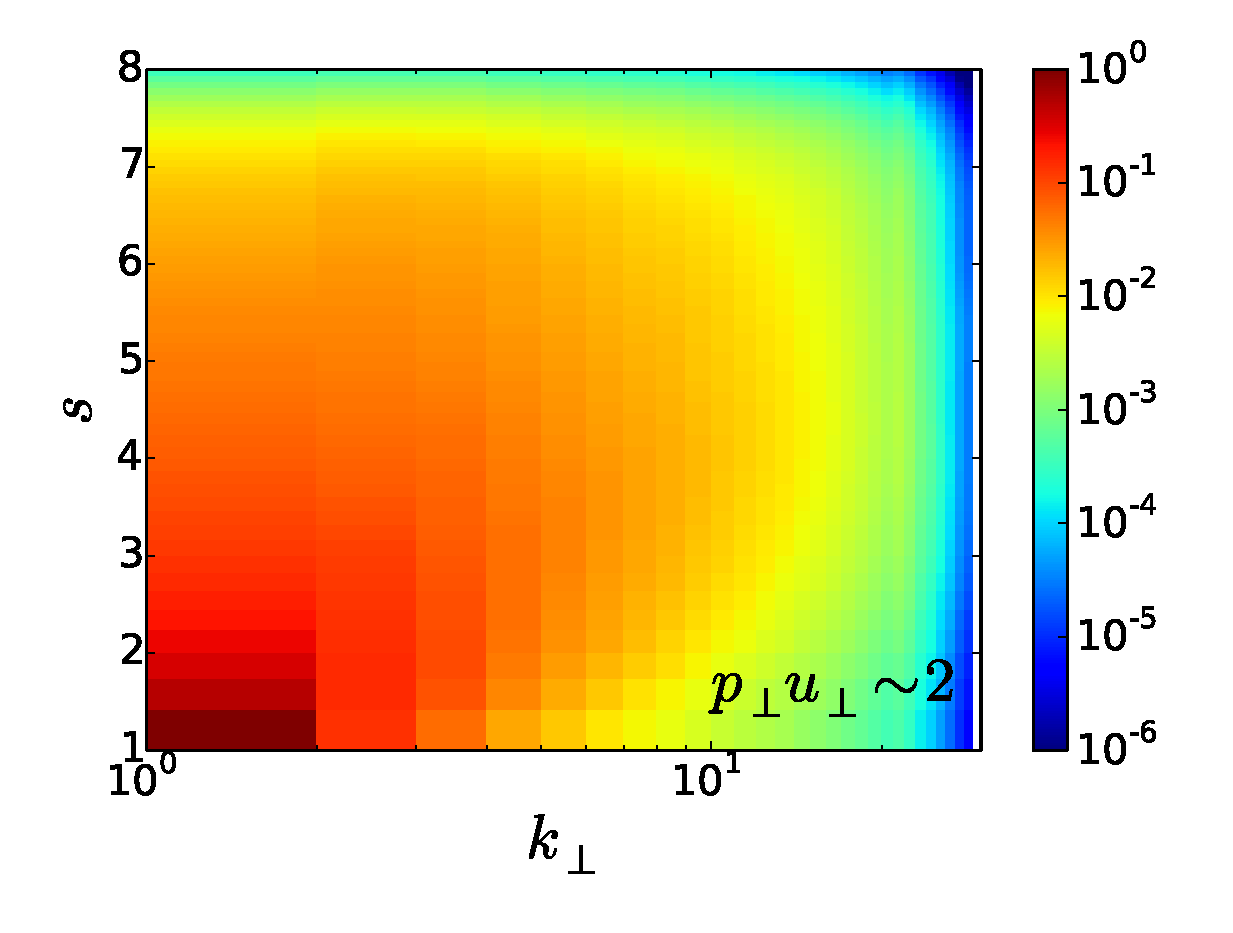
\includegraphics[width=7.4cm]{figs/phmixnlpp0/M100_2_vsskp.eps}
        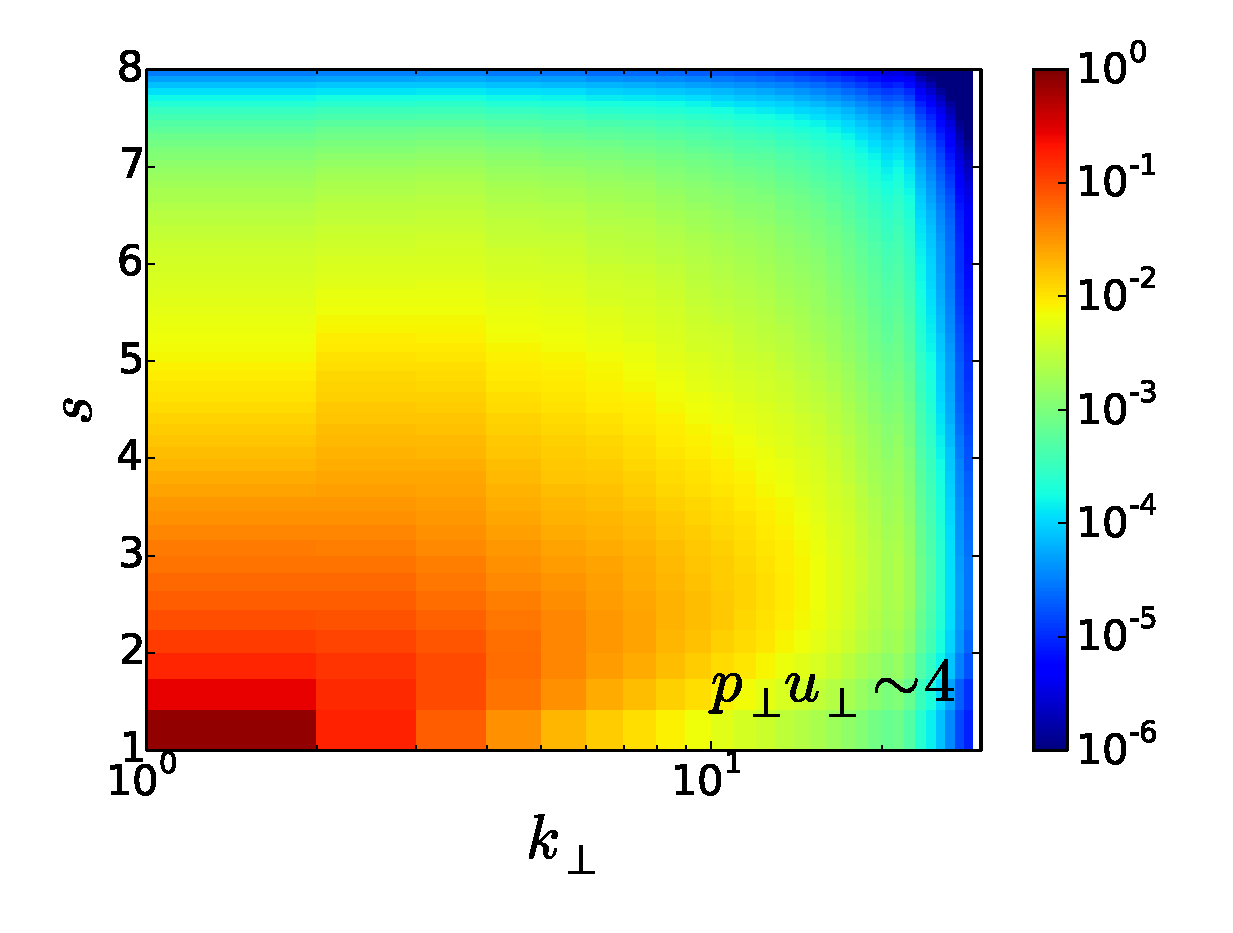
\includegraphics[width=7.4cm]{figs/phmixnlpp0/M100_4_vsskp.eps}

        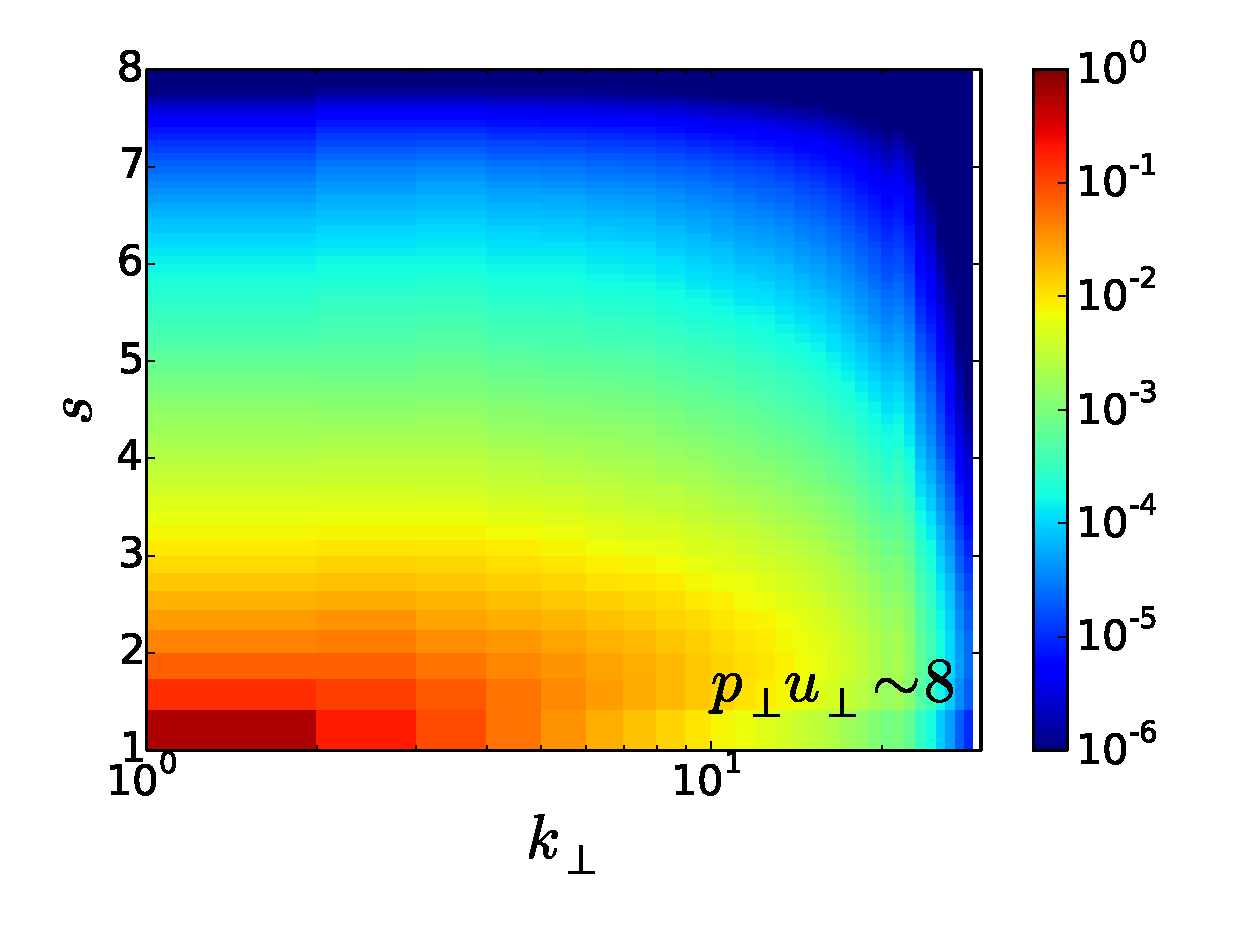
\includegraphics[width=7.4cm]{figs/phmixnlpp0/M100_8_vsskp.eps}
        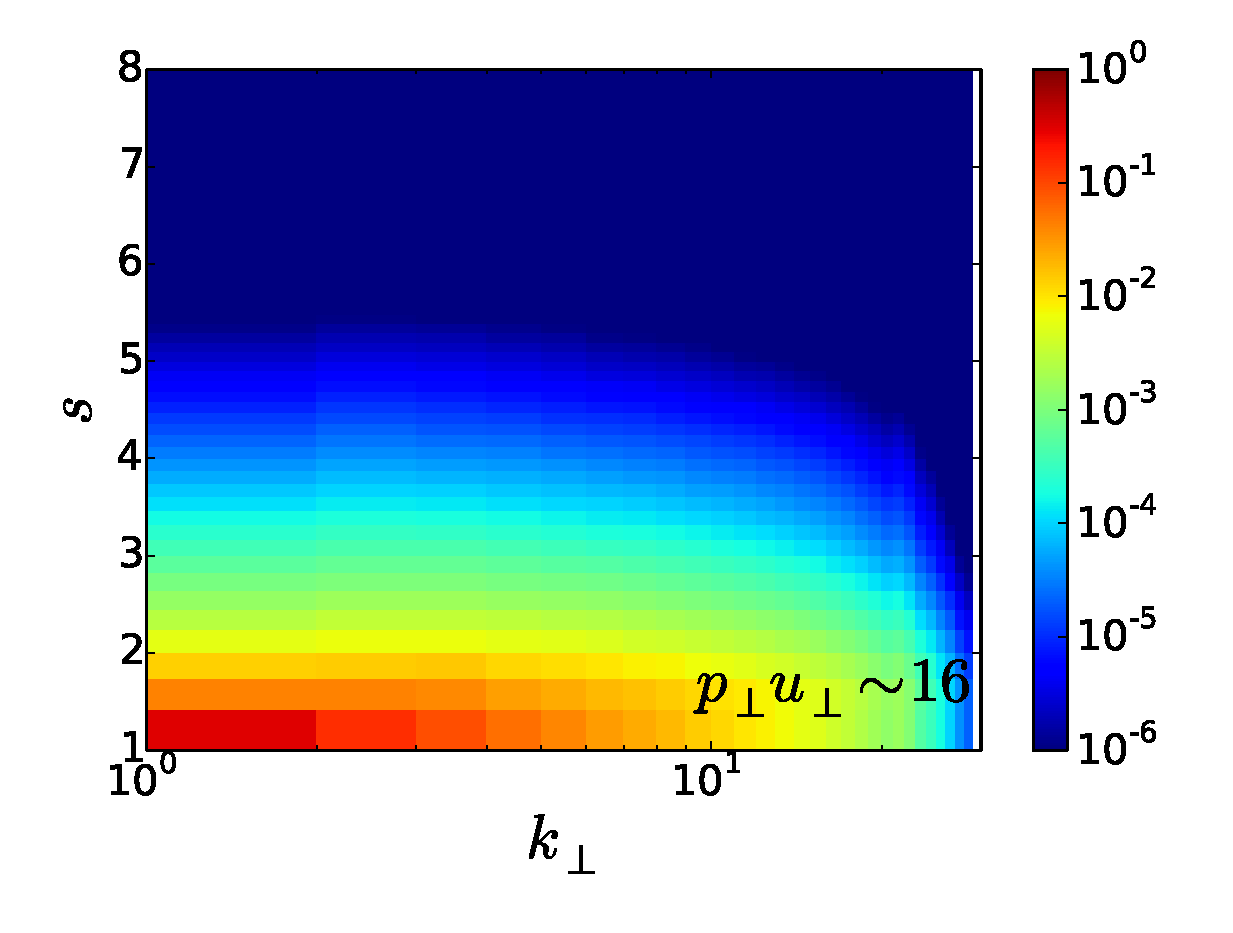
\includegraphics[width=7.4cm]{figs/phmixnlpp0/M100_16_vsskp.eps}
        \caption{The spectrum $\Fsk$ vs $s-k_\perp$ at $\kpar=1$, for four different 
        $\pu$.
        For larger values of $\pu$, the spectrum does not extend far into Hermite space, as expected.}
        \label{pp0:fig:vsskp}
    \end{center}
    \end{figure}

    We observe in our simulations, that when the nonlinear timescale is faster than the linear timescale, the passive scalar
    does not get phase-mixed. This is shown in \figref{pp0:fig:vsskp}, where we see
    the spread of the spectrum in $s$ to be strongly dependent on the strength of the
    nonlinearity. \Figsand{pp0:fig:vss}{pp0:fig:fixkpvss} show this dependence---the spectrum decays exponentially in
    $s$ at a rate proportional to $\pu/k_{\parallel0}\vth$. 
    \begin{figure}
    \begin{center}
        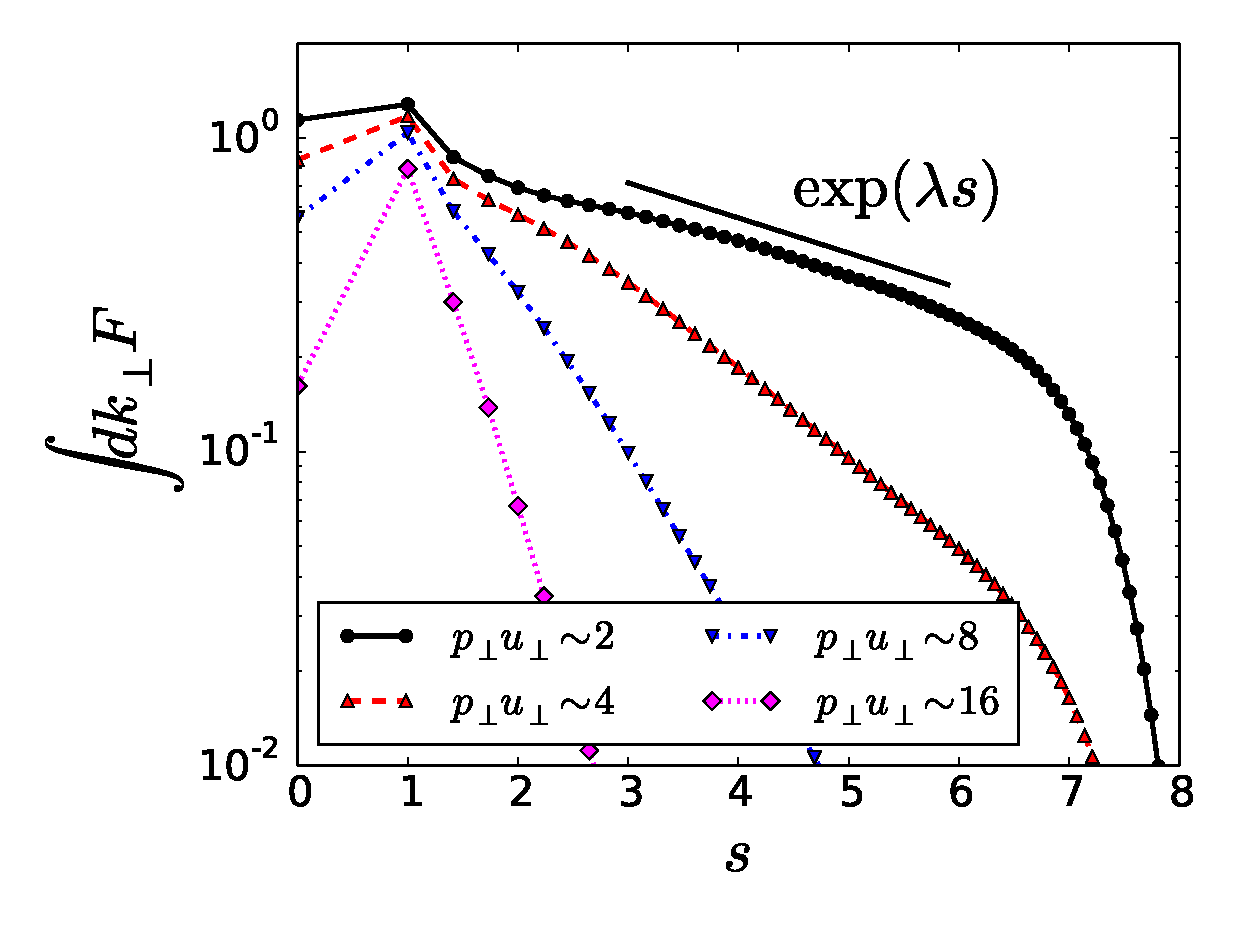
\includegraphics[width=7.4cm]{figs/phmixnlpp0/M100_vss.eps}
        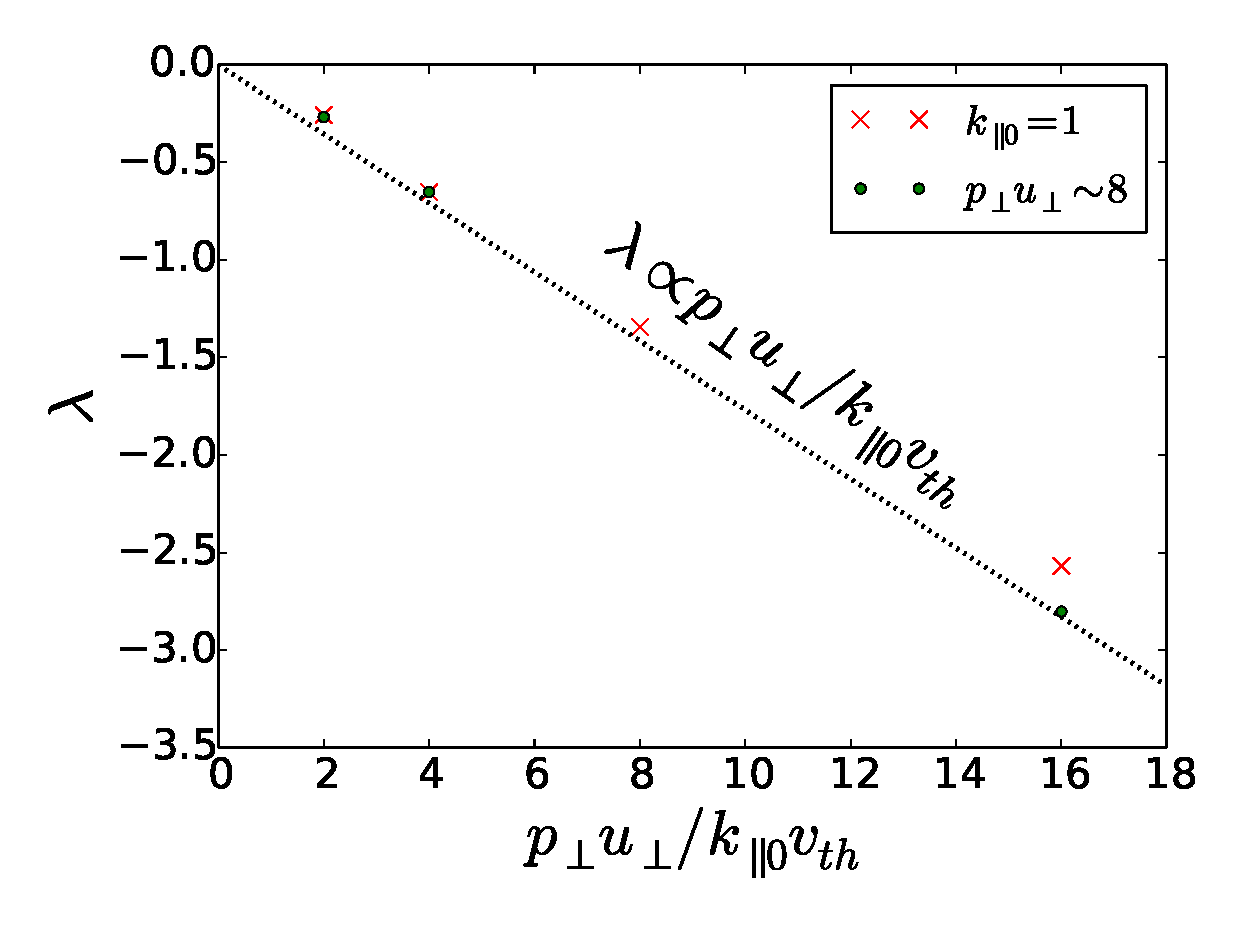
\includegraphics[width=7.4cm]{figs/phmixnlpp0/lambda_vs_gperp.eps}
        \caption{The 1D spectrum $\int dk_\perp \Fsk$ vs $s$ (left) is seen to be an exponential
        decay at a rate $\lambda$ proportional to $\pu/k_{\parallel0}\vth$. The decay rate
        is plotted versus $\pu/k_{\parallel0}\vth$ on the right---the red crosses are
        runs with fixed $k_{\parallel0}=1$ and varying $\pu$, whereas the green circles
        are runs with fixed $\pu \sim 8$ and varying $k_{\parallel0}$.}
        \label{pp0:fig:vss}
    \end{center}
    \end{figure}
    \begin{figure}
    \begin{center}
        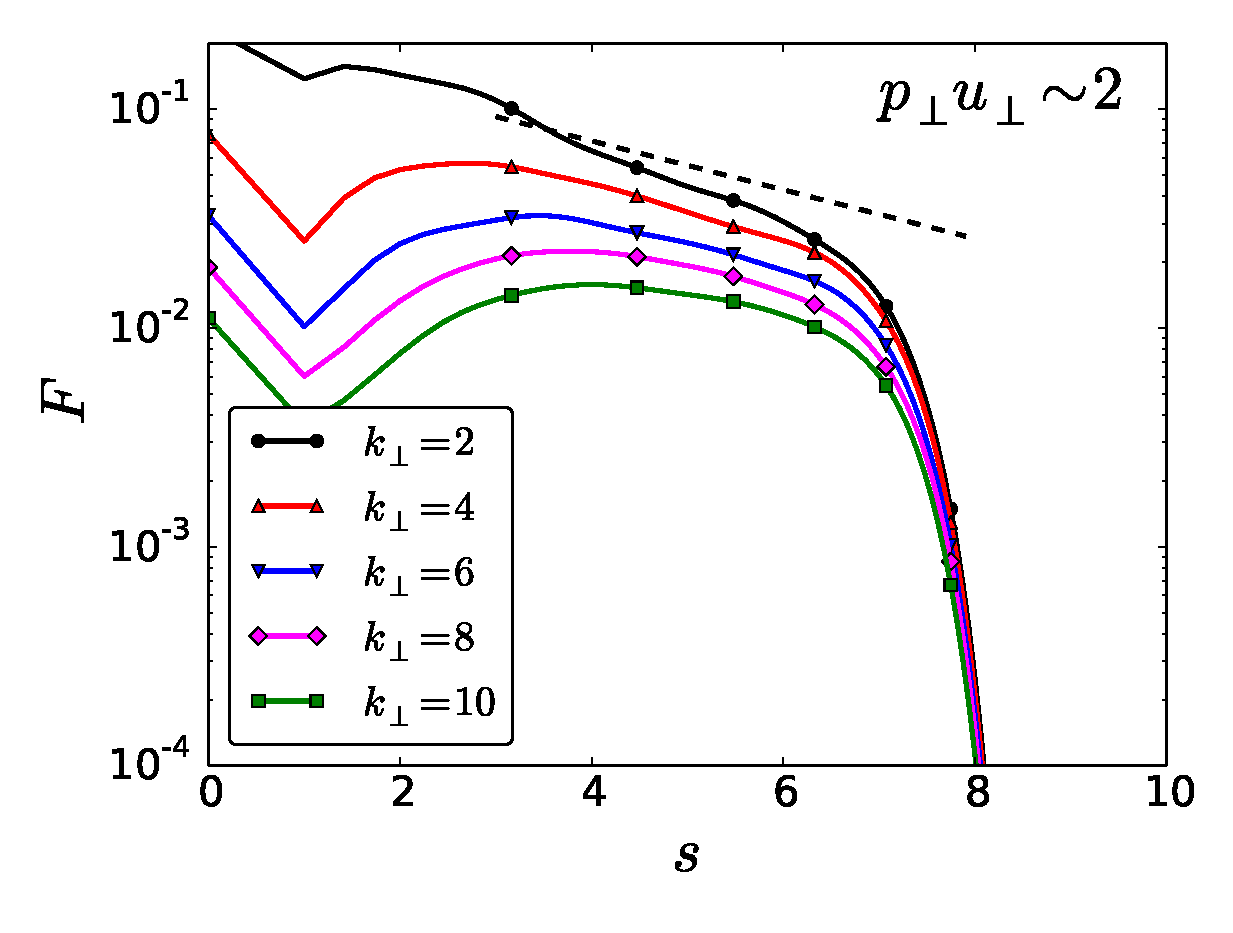
\includegraphics[width=7.4cm]{figs/phmixnlpp0/M100_2_fixkp_vss.eps}
        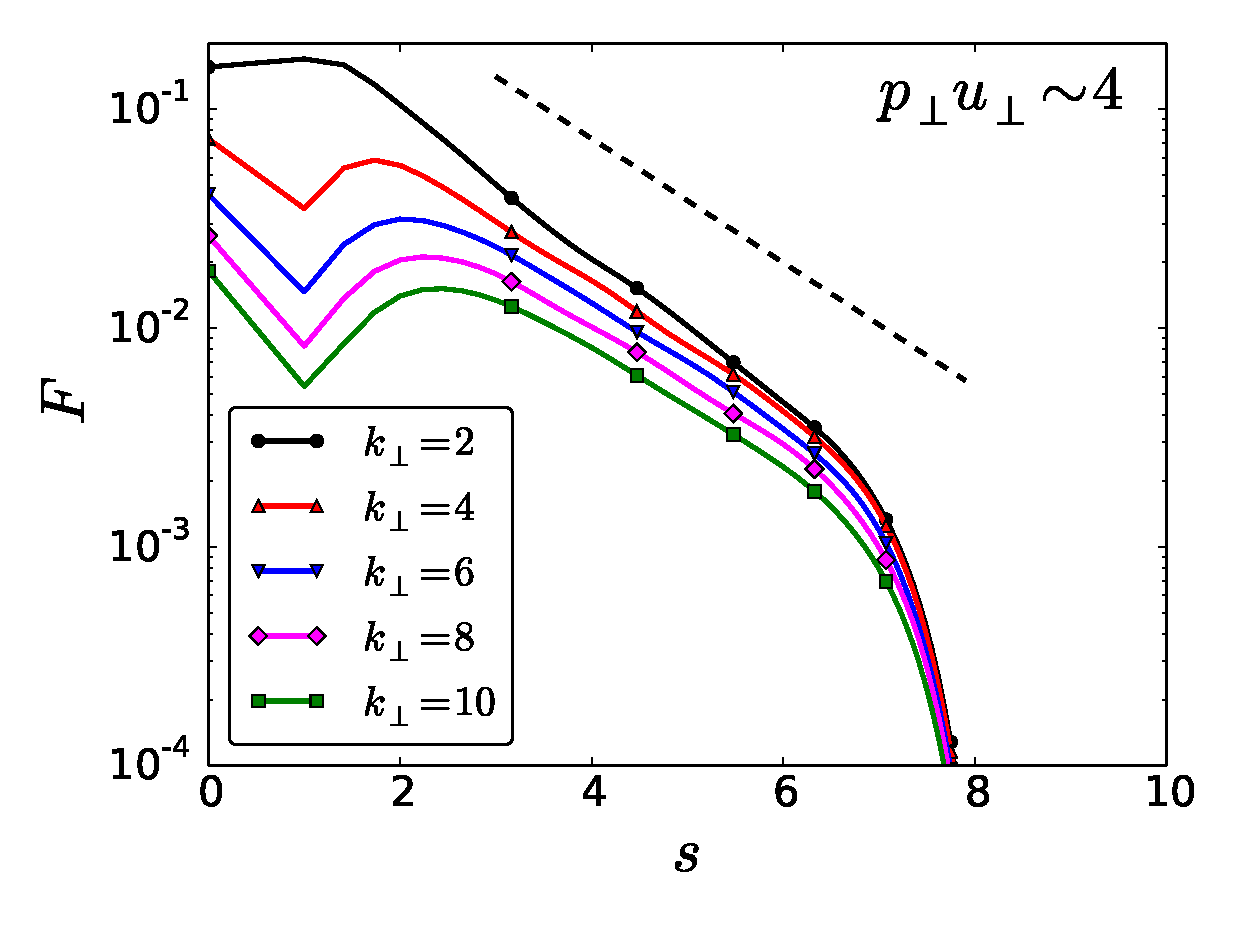
\includegraphics[width=7.4cm]{figs/phmixnlpp0/M100_4_fixkp_vss.eps}

        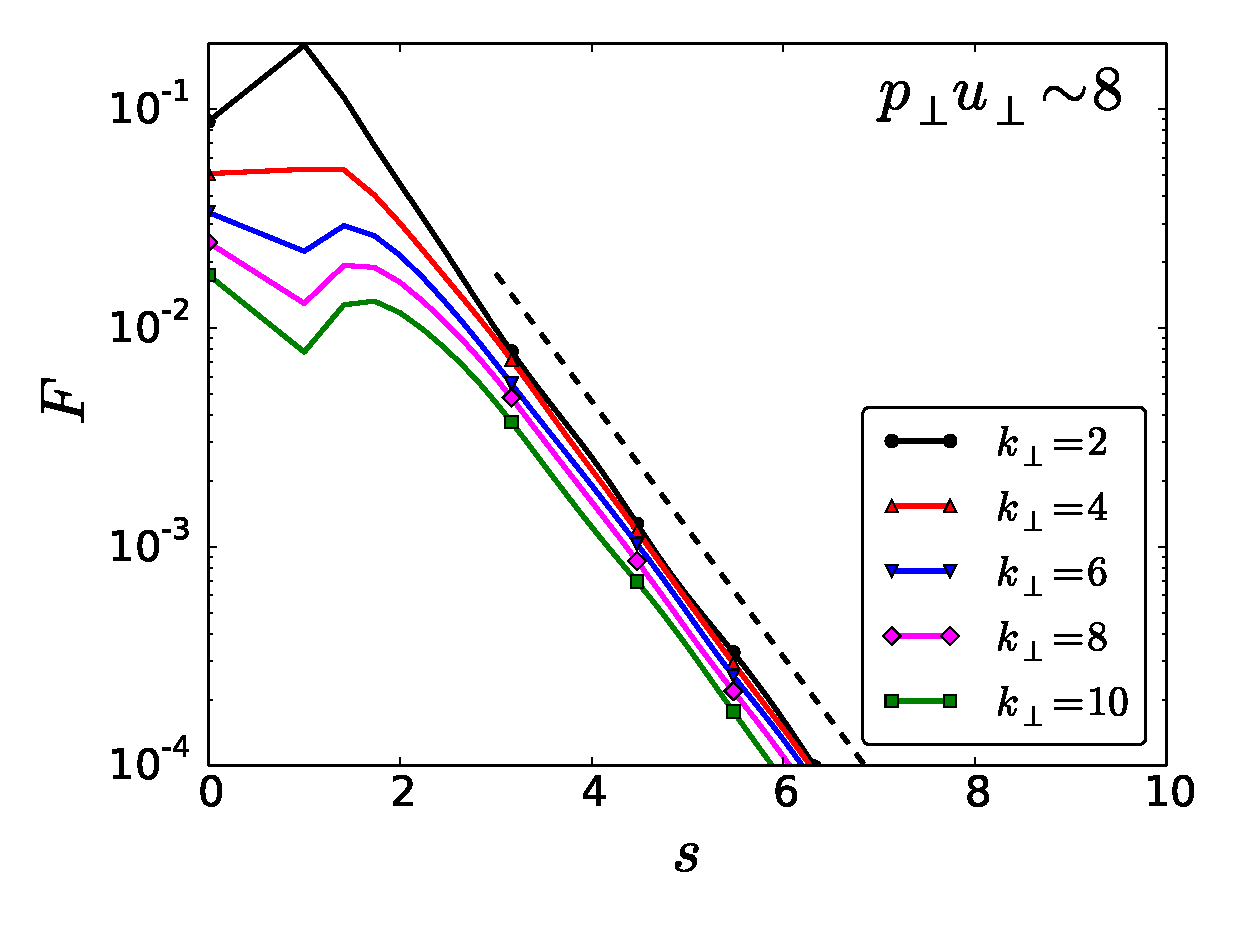
\includegraphics[width=7.4cm]{figs/phmixnlpp0/M100_8_fixkp_vss.eps}
        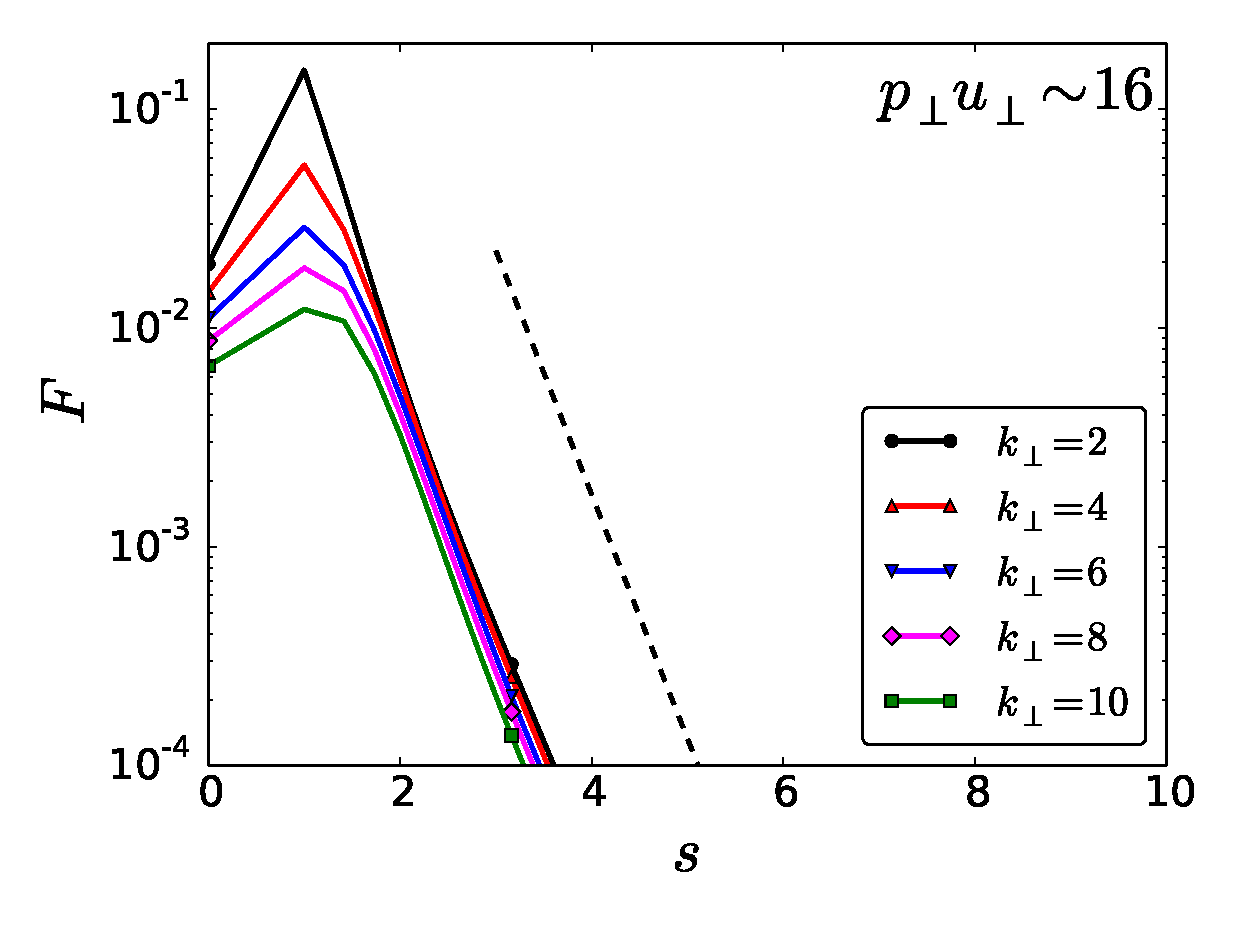
\includegraphics[width=7.4cm]{figs/phmixnlpp0/M100_16_fixkp_vss.eps}
        \caption{Spectrum $F$ at fixed $k_\perp$ vs $s$ for four different values of
        $\pu$.
        After an initial ``transient" in $s$, the spectrum decays exponentially at a
        rate $\propto \pu/k_{\parallel0} \vth$---the dashed line depicts the
        expected spectrum.}
        \label{pp0:fig:fixkpvss}
    \end{center}
    \end{figure}
    This is further confirmed by \figref{pp0:fig:vskp}, where the passive scalar is shown
    to have a perpendicular spectrum consistent with the fluid limit.
    \begin{figure}
    \begin{center}
        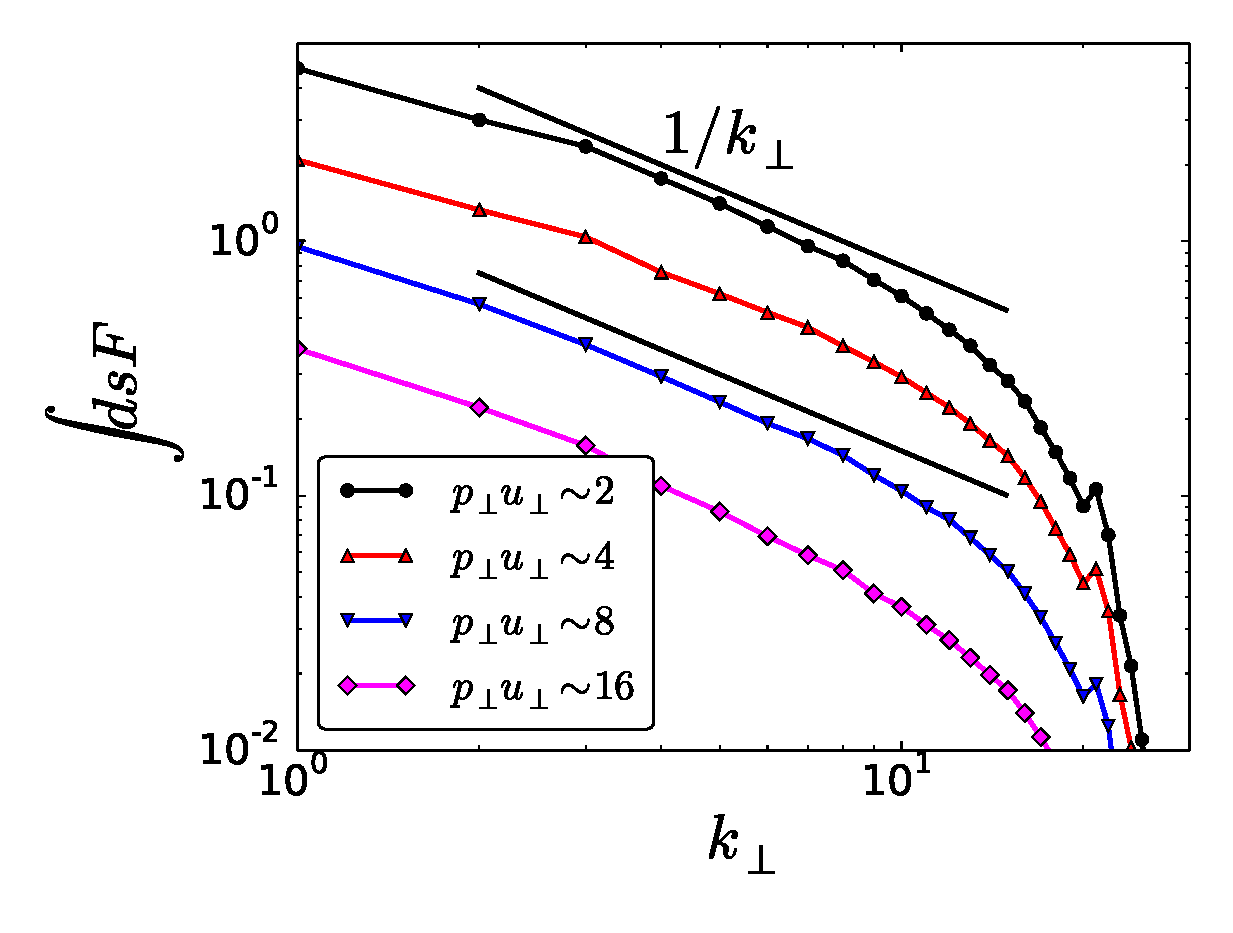
\includegraphics[width=14.8cm]{figs/phmixnlpp0/M100_vskp.eps}
        \caption{1D spectrum $\int ds \Fsk$ vs $k_\perp$. The spectrum becomes
        increasingly fluid-like ($\sim1/k_\perp$), as $\pu$ is increased.}
        \label{pp0:fig:vskp}
    \end{center}
    \end{figure}

    In \figref{pp0:fig:normcoll} we plot the dissipation due to collisions normalized to the
    total dissipation (collisional and diffusion) as a function of $\pu/k_{\parallel0}\vth$,
    where we see that the dissipation due to collisions decreases
    exponentially as the nonlinear advection rate is increased with respect to the linear
    frequency, i.e., once nonlinear, the system preferentially dissipates via diffusion.
    
    \begin{figure}
    \begin{center}
        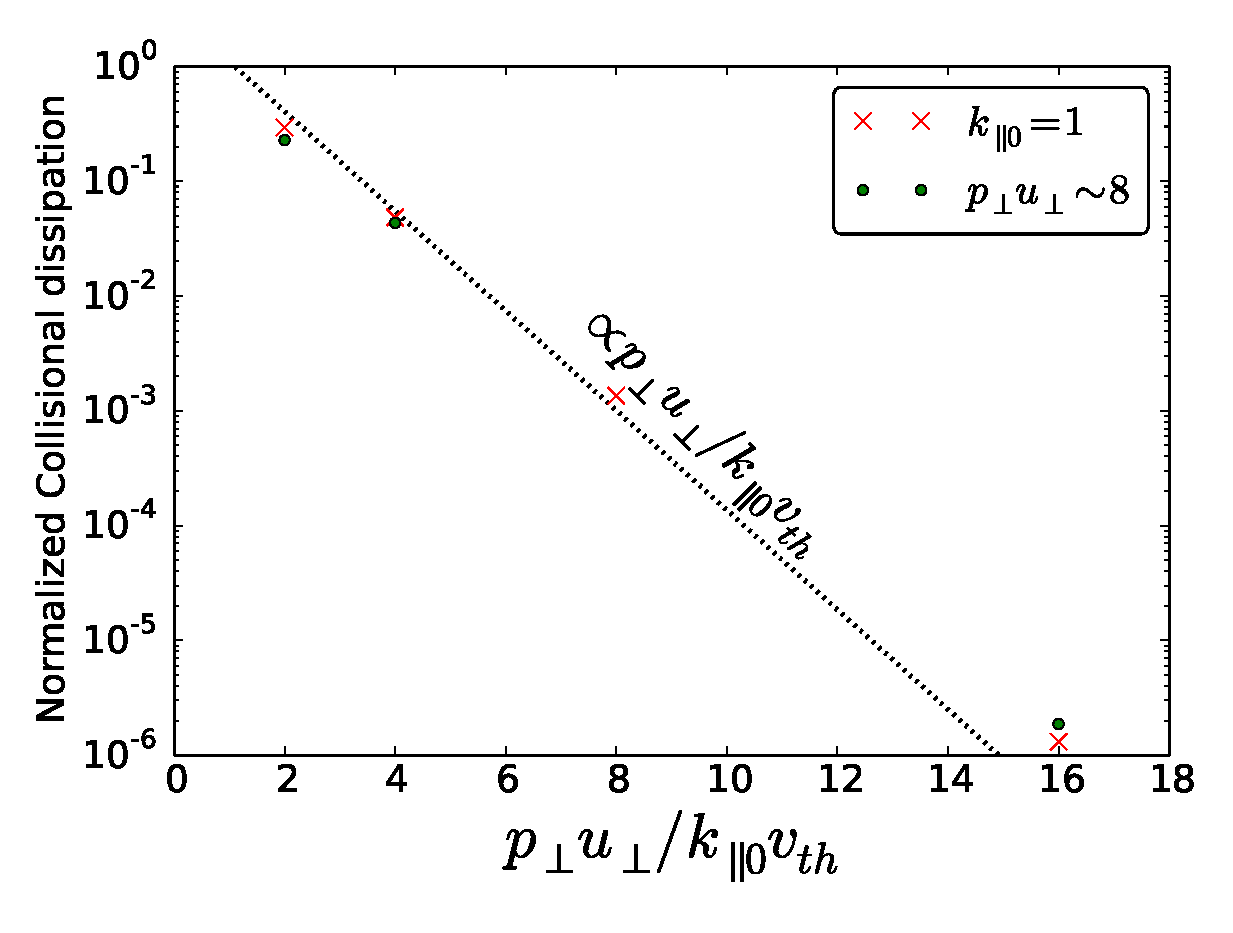
\includegraphics[width=14.8cm]{figs/phmixnlpp0/M100_normcoll.eps}
        \caption{Collisional dissipation normalized to the total dissipation vs
        $\pu/k_{\parallel0\vth}$. As the system becomes more nonlinear, most of
        the energy is dissipated by the diffusive cutoff, and vanishingly small amount of energy is dissipated
        via the collisional channel.}
        \label{pp0:fig:normcoll}
    \end{center}
    \end{figure}

\section{Discussion}
    We showed by numerically solving \eqsdash{pp0:eq:driftkin}{pp0:eq:boltz}, that if a
    kinetic passive scalar is being advected by a 2D velocity field, in the strongly
    nonlinear regime, the steady-state
    behavior is fluid-like. The nonlinear cascade
    transfers the energy to finer perpendicular
    scales, not allowing the scalar to phase mix. As a result, the perpendicular spectrum
    for such a system in the Batchelor limit is the well-known fluid spectrum:
    $1/k_\perp$. The spectrum in Hermite space decays exponentially at
    the rate $\pu/k_{\parallel0}\vth$, which is consistent with the fluid-like behavior of
    the system. 
    The dissipation for
    such a system happens almost completely through diffusion, since negligible
    amount of energy is transferred to small scales in velocity space, which makes
    collisions inaccessible.

    It has been suggested that the compressive fluctuations in the solar wind do not
    undergo a parallel cascade \cite{tome} (see \secref{slowmodes:sec:intro} for a
    detailed discussion). If this is assumed to be true, then the results presented in
    this chapter help explain the observed power law spectra of density fluctuations. In
    KRMHD, the nonlinear cascade rate associated with the background Alfv\'{e}nic
    turbulence increases with the perpendicular wavenumber; whereas, in absence of a
    parallel cascade, the linear
    phase mixing rate of the compressive fluctuations remains unchanged. As a result, beyond a certain scale the nonlinear
    cascade dominates, and disallows the slow modes to phase mix, resulting in a
    fluid-like turbulent cascade, \ie, power law spectra.
    
    The results discussed in this chapter are the kinetic generalization of the Batchelor spectrum for a 
    passive scalar, where the advecting velocity is 2D and the scalar does not undergo a
    parallel cascade. We discuss the effects of parallel cascade in the next chapter, by
    considering a 3D advecting velocity field.
    
